% CS4234 mini-project report: Linear Programming and Total Unimodularity.
% Format (course rule, do not change): single column, 11pt, main body at most
% 10 pages; anything beyond goes in the appendix.
% Build (from this folder): tectonic -k -o build main.tex  ->  build/main.pdf
\documentclass[11pt,a4paper]{article}

\usepackage[margin=2.5cm]{geometry}
\usepackage[T1]{fontenc}
\usepackage{lmodern}
\usepackage{microtype}
\usepackage{amsmath,amssymb,amsthm}
\usepackage{graphicx}
\usepackage{booktabs}
\usepackage{xcolor}
\usepackage{tikz}
\usetikzlibrary{arrows.meta,calc,positioning}
\usepackage{pgfplots}
\pgfplotsset{compat=1.18}
\usepackage{caption}
\captionsetup{font=small,labelfont=bf}
\usepackage{algorithm}
\usepackage[noend]{algpseudocode}
\usepackage{enumitem}
\usepackage{pdflscape}
\usepackage{rotating}
\usepackage{float}
\usepackage[numbers,sort&compress]{natbib}
\usepackage[hidelinks]{hyperref}

% Colours with the same meaning as on the slides (slides/theme.css).
\definecolor{good}{HTML}{1F7A4D}    % integral / TU / works
\definecolor{warn}{HTML}{B4531A}    % fractional / not TU / fails
\definecolor{accent}{HTML}{2457C5}  % highlights
\definecolor{muted}{HTML}{5F6368}   % secondary text
% Chart series (validated categorical palette): LP, compiled, pure Python.
\definecolor{series1}{HTML}{2A78D6}
\definecolor{series2}{HTML}{EB6834}
\definecolor{series3}{HTML}{1BAF7A}
% Legend sample for the E4 plot: \legline{colour}{mark}.
\newcommand{\legline}[2]{\tikz[baseline=-0.6ex]{%
  \draw[#1, line width=1pt] (0,0) -- (0.6,0);
  \draw[#1] plot[only marks, mark=#2, mark size=2pt] coordinates {(0.3,0)};}}

% Notation (README Section 4).
\newcommand{\R}{\mathbb{R}}
\newcommand{\Z}{\mathbb{Z}}
\newcommand{\optlp}{\mathrm{OPT}_{\mathrm{LP}}}
\newcommand{\optilp}{\mathrm{OPT}_{\mathrm{ILP}}}

\theoremstyle{plain}
\newtheorem{theorem}{Theorem}
\newtheorem{lemma}[theorem]{Lemma}
\newtheorem{corollary}[theorem]{Corollary}
\theoremstyle{definition}
\newtheorem{definition}[theorem]{Definition}

\setlist{itemsep=2pt,topsep=4pt}
% Compact bullets for the experiment setups (E1--E4).
\newlist{setup}{itemize}{1}
\setlist[setup]{label=\textbullet, leftmargin=1.2em, topsep=1pt, itemsep=0pt, parsep=0pt}

% Compact, uniform spacing for run-in paragraph headings and floats.
\makeatletter
\renewcommand\paragraph{\@startsection{paragraph}{4}{\z@}%
  {1.6ex \@plus .4ex \@minus .2ex}{-1em}{\normalfont\normalsize\bfseries}}
\makeatother
\setlength{\textfloatsep}{12pt plus 2pt minus 4pt}
\setlength{\floatsep}{10pt plus 2pt minus 2pt}
\setlength{\intextsep}{10pt plus 2pt minus 2pt}
\captionsetup{skip=6pt}
\captionsetup[table]{position=top}

% Pseudocode: every algorithm is a ruled box set with \captionof, so that two
% can sit side by side inside one figure. Usage: \begin{algobox}{Title}{label}.
\captionsetup[algorithm]{labelsep=colon,singlelinecheck=false}
\algrenewcommand\algorithmicrequire{\textbf{Input:}}
\algrenewcommand\algorithmicensure{\textbf{Output:}}
\algrenewcommand\algorithmiccomment[1]{\hfill\textcolor{muted}{$\triangleright$ #1}}
\newenvironment{algobox}[2]{%
  \par\noindent\rule{\linewidth}{0.8pt}\par\vspace{-4pt}
  \captionof{algorithm}{#1}\label{#2}\vspace{-9pt}
  \noindent\rule{\linewidth}{0.4pt}\par\vspace{-4pt}
  \small\begin{algorithmic}[1]}{%
  \end{algorithmic}\vspace{-6pt}\noindent\rule{\linewidth}{0.8pt}\par}

\title{Linear Programming and Total Unimodularity\\[4pt]
  \large When does an LP relaxation solve an integer program exactly?}
% Authors in presenter order (P1-P4), each with their student number.
\author{%
  \begin{tabular}{@{}cccc@{}}
    Wong Yee Hern & Teo Yock Cheng & Feilin Liangga Putri & Daryl Koh Han Boon \\
    \small A0307067E & \small A0271666W & \small A0307092J & \small A0272260M
  \end{tabular}\\[8pt]
  \small CS4234 Optimization Algorithms, National University of Singapore, AY2026/27 Semester~1}
\date{November 2026}

\begin{document}
\maketitle

\section{Introduction}\label{sec:intro}

Many optimisation problems are \emph{integer linear programs} (ILPs): a linear objective and linear constraints over integer variables. Solving an ILP is NP-hard in general \cite{karp1972}, whereas a \emph{linear program} (LP) can be solved in polynomial time \cite{khachiyan1979}. A standard approximation recipe exploits this gap: write the problem as an ILP, drop integrality to get the \emph{LP relaxation}, solve it and round. For a minimisation problem the relaxation can only lower the optimum, $\optlp \le \optilp$, so rounding usually costs something. For vertex cover, rounding at $\tfrac12$ only guarantees a factor of~2 \cite{hochbaum1982}.

Sometimes rounding costs nothing. The \emph{vertex cover LP} (VC LP) of a graph $G=(V,E)$ is
\[
  \min \sum_{v\in V} x_v
  \quad\text{s.t.}\quad x_u + x_v \ge 1 \ \text{ for every } \{u,v\}\in E,
  \qquad 0 \le x \le 1 .
\]
On the triangle $C_3$ the all-$\tfrac12$ point is optimal with value $1.5$ (summing the edge constraints gives $2\sum_v x_v\ge3$), but every cover needs two vertices. On the 4-cycle $C_4$ the LP optimum is~$2$, and simplex returns an integral cover (Figure~\ref{fig:running}). This report asks three questions:

\begin{quote}\itshape
  When does solving an LP give an integer optimum? How do we recognise such problems? Does the LP algorithm we use matter?
\end{quote}

\begin{figure}[H]
  \centering
  % Figure~\ref{fig:running}: VC LP on C_3 and C_4.
% Input by sections/01-introduction.tex.
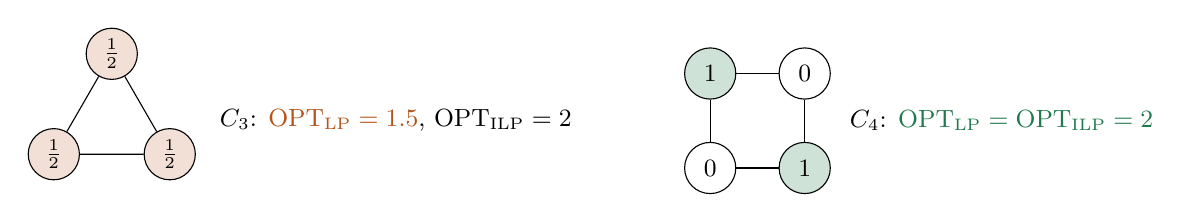
\begin{tikzpicture}[
    vtx/.style={circle, draw, minimum size=6.5mm, inner sep=0pt, font=\small},
    lbl/.style={font=\small}]
  \begin{scope}
    \node[vtx, fill=warn!18] (a) at (90:0.85)  {$\tfrac12$};
    \node[vtx, fill=warn!18] (b) at (210:0.85) {$\tfrac12$};
    \node[vtx, fill=warn!18] (c) at (330:0.85) {$\tfrac12$};
    \draw (a) -- (b) -- (c) -- (a);
    \node[lbl, anchor=west] at (1.25,0) {$C_3$: \textcolor{warn}{$\optlp = 1.5$}, $\optilp = 2$};
  \end{scope}
  \begin{scope}[xshift=8.2cm]
    \node[vtx, fill=good!22] (p) at (-0.6, 0.6) {$1$};
    \node[vtx]               (q) at ( 0.6, 0.6) {$0$};
    \node[vtx, fill=good!22] (r) at ( 0.6,-0.6) {$1$};
    \node[vtx]               (s) at (-0.6,-0.6) {$0$};
    \draw (p) -- (q) -- (r) -- (s) -- (p);
    \node[lbl, anchor=west] at (1.05,0) {$C_4$: \textcolor{good}{$\optlp = \optilp = 2$}};
  \end{scope}
\end{tikzpicture}%

  \caption{The running example, labelled with optimal LP solutions $x_v$. On $C_3$ the LP optimum is fractional and below the integer optimum; on $C_4$ simplex returns an integral optimal cover.}
  \label{fig:running}
\end{figure}

The answer centres on \emph{total unimodularity} (TU): every square submatrix of the constraint matrix $A$ has determinant $-1$, $0$ or~$1$. If $A$ is TU and the right-hand side $b$ is integral, every vertex of the feasible region is integral \cite{hoffman1956}, so the LP has an integral optimum. The matrix of $C_4$ is TU because $C_4$ is bipartite; that of $C_3$ is not, since its determinant is~$2$.

\paragraph{Scope and outline.} Figure~\ref{fig:roadmap} maps the questions to our sections and experiments. We prove the direction of the Hoffman--Kruskal theorem that we use, derive the main TU families, compare three ways to recognise TU, and study how LP algorithms behave on these LPs. We state Seymour's theorem \cite{seymour1980} without proof and use an existing implementation of its test, and only mention total dual integrality and the non-bipartite matching polytope. All code, data and raw results are in our repository.\footnote{\url{https://github.com/feilinlp/linear-programming-total-unimodularity}} Every number in this report was produced there, and each experiment reruns with one command (Appendix~\ref{app:repro}).

\begin{figure}[H]
  \centering
  % Figure~\ref{fig:roadmap}: questions, theory and experiments.
% Input by sections/01-introduction.tex.
\begin{tikzpicture}[font=\small,
    q/.style={rectangle, rounded corners=2pt, fill=accent!12, draw=accent!60,
              text width=4.85cm, align=center, inner sep=3pt, minimum height=7mm},
    th/.style={rectangle, draw=black!25, text width=4.85cm, align=flush left,
               inner sep=3pt, minimum height=13mm},
    ex/.style={rectangle, rounded corners=2pt, fill=black!6, draw=black!25,
               text width=4.85cm, align=flush left, inner sep=3pt, minimum height=10.5mm}]
  \foreach \x/\name/\qq/\theory/\exper in {
      0/1/{\textbf{When} is the LP exact?}/{\S\ref{sec:tu}: Hoffman--Kruskal \cite{hoffman1956}, TU families, half-integrality \cite{nemhauser1975}}/{\textbf{E1}: is TU necessary?},
      5.35/2/{\textbf{How} do we recognise TU?}/{\S\ref{sec:recognise}: brute force, Ghouila-Houri \cite{ghouilahouri1962}, Seymour \cite{seymour1980}}/{\textbf{E2}: how costly is recognition?},
      10.7/3/{Does the \textbf{algorithm} matter?}/{\S\ref{sec:solve}: simplex \cite{dantzig1951}, ellipsoid \cite{khachiyan1979}, IPM \cite{karmarkar1984}, crossover \cite{megiddo1991}}/{\textbf{E3}: which optimal point?\\ \textbf{E4}: LP or specialised code?}} {
    \node[q]  (q\name) at (\x, 0) {\qq};
    \node[th, below=1mm of q\name.south, anchor=north] (t\name) {\theory};
    \node[ex, below=1mm of t\name.south, anchor=north] (e\name) {\exper};
  }
\end{tikzpicture}%

  \caption{Roadmap: the three questions, the theory and main papers that answer each, and the experiments that test them.}
  \label{fig:roadmap}
\end{figure}

\section{Preliminaries}\label{sec:prelim}

\paragraph{Linear programs.} An LP in standard form is $\max\ c^\top x$ s.t.\ $Ax \le b$, $x \ge 0$, with constraint matrix $A\in\R^{m\times n}$ ($m$ constraints, $n$ variables), right-hand side $b\in\R^m$ and objective $c\in\R^n$. Its dual is $\min\ b^\top y$ s.t.\ $A^\top y \ge c$, $y \ge 0$, and when both are feasible their optima are equal (strong duality) \cite{bertsimas1997}. Minimisation, $\ge$ rows, equalities and bounds reduce to this form by negating and adding rows; Lemma~\ref{lem:ops} shows that this preserves TU. $L$ is the number of bits needed to write down $A$, $b$ and~$c$.

\paragraph{Vertices and bases.} A point of the polyhedron $P=\{x : A'x\le b'\}$ (with $x\ge 0$ among the rows) is a \emph{vertex} if it is not the midpoint of two other points of $P$; equivalently, it is the unique solution of $n$ linearly independent constraints tight at it. A feasible, bounded LP over such a $P$ has an optimal vertex \cite{bertsimas1997}. Simplex works in equality form $[A\ \ I]\,\bar x = b$, $\bar x\ge 0$ (with slack variables). A \emph{basis} $B$ is a set of $m$ linearly independent columns of $[A\ \ I]$, $A_B$ is the corresponding square submatrix, and the basic solution sets $x_B = A_B^{-1}b$ and all other variables to~$0$. The basic feasible solutions are exactly the vertices.

\paragraph{Exact versus integral.} The ILP adds $x\in\Z^n$. We call the relaxation \emph{exact} if $\optlp = \optilp$, and an LP solution \emph{integral} if all its coordinates are integers. An integral optimal LP solution proves exactness, but an exact LP can also have fractional optimal solutions. E1 and E3 measure the two properties separately.

\paragraph{Total unimodularity.} $A$ is TU if every square submatrix (any $k$ rows and any $k$ columns) has determinant in $\{-1,0,1\}$. In particular every entry is $-1$, $0$ or $1$, and TU depends on $A$ alone, not on $b$ or $c$. The VC LP's matrix is the \emph{incidence matrix} of the graph: one row per edge, one column per vertex, and a $1$ where the vertex is an endpoint of the edge. (In graph contexts $n=|V|$ and $m=|E|$, which here agrees with the LP convention.) With edges in cyclic order, $A_{C_3}$ has rows $(1,1,0)$, $(0,1,1)$, $(1,0,1)$ and determinant~$2$, so it is not TU. $A_{C_4}$ (Figure~\ref{fig:families}a) has determinant~$0$, and Section~\ref{sec:families} shows that all its square submatrices have determinant in $\{-1,0,1\}$. $C_k$ denotes the cycle on $k$ vertices.

\section{Total unimodularity and integral optima}\label{sec:tu}

\subsection{The Hoffman--Kruskal theorem}\label{sec:hk}

Real LPs add bounds, equalities and sign constraints to $A$. The first lemma shows that these keep a matrix TU.

\begin{lemma}\label{lem:ops}
  If $A$ is TU, then so are $A^\top$, any matrix obtained from $A$ by permuting or negating rows or columns, and $A$ with an extra row that is a unit vector $e_j^\top$ or $\pm$ a copy of a row of $A$. In particular, $\bigl[A;\,-A;\,I;\,-I\bigr]$ is TU, so equalities $Ax=b$ and bounds $\ell\le x\le u$ keep a system TU.
\end{lemma}
\begin{proof}
  Transposing and permuting do not change $|\det|$, and negating a row or column flips its sign. In a square submatrix $M$ of the extended matrix, a part of a unit row lets us expand along it (induction on the size of $M$); a row together with $\pm$ its copy gives $\det M=0$; otherwise $M$ is, up to row signs, a submatrix of~$A$.
\end{proof}

\begin{theorem}[Hoffman--Kruskal \cite{hoffman1956}]\label{thm:hk}
  Let $A$ be an integral matrix. Then $A$ is TU if and only if, for every integral vector $b$, every vertex of $\{x : Ax\le b,\ x\ge 0\}$ is integral.
\end{theorem}
\begin{proof}[Proof of ``only if'']
  Let $A$ be TU and $b$ integral. By Lemma~\ref{lem:ops} we may fold $x\ge 0$ into the rows, so let $x^*$ be a vertex of $P=\{x : Ax\le b\}$. Then $x^*$ is the unique solution of $A'x=b'$, where $A'$ consists of $n$ linearly independent rows of $A$ tight at $x^*$ and $b'$ is the matching part of $b$. As a nonsingular square submatrix of a TU matrix, $A'$ has $\det A'=\pm1$. By Cramer's rule, $x^*_j = \det A'_j / \det A'$, where $A'_j$ is $A'$ with column $j$ replaced by $b'$. Since $A'_j$ is integral, $x^*_j = \pm\det A'_j\in\Z$.
\end{proof}

We omit the converse \cite{schrijver1986}. It needs integral vertices for \emph{every} integral $b$, so a non-TU matrix can still give an integral optimum for one particular $b$ and $c$ (Section~\ref{sec:e1}). Figure~\ref{fig:hk} shows the difference, and the consequence we use throughout is:

\begin{corollary}\label{cor:lp-exact}
  If $A$ is TU and $b$, $\ell$, $u$ are integral, then for every objective $c$, the LP $\max\{c^\top x : Ax\le b,\ \ell\le x\le u\}$, if it has an optimum, has an integral optimal vertex. Simplex returns a vertex, so it returns an integral optimum, and the relaxation is exact.
\end{corollary}

\begin{figure}[H]
  \centering
  % Figure~\ref{fig:hk}: TU vs non-TU feasible regions.
% Input by sections/03-tu-integrality.tex.
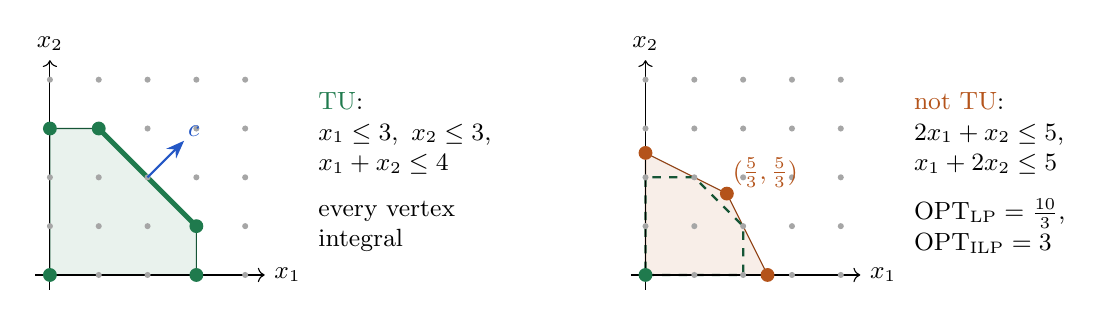
\begin{tikzpicture}[scale=0.62, font=\small,
    lat/.style={circle, fill=black!35, inner sep=0pt, minimum size=2.2pt},
    gv/.style={circle, fill=good, inner sep=0pt, minimum size=5pt},
    wv/.style={circle, fill=warn, inner sep=0pt, minimum size=5pt}]
  \begin{scope}
    \fill[good!10] (0,0) -- (3,0) -- (3,1) -- (1,3) -- (0,3) -- cycle;
    \draw[good!70!black] (0,0) -- (3,0) -- (3,1) -- (1,3) -- (0,3) -- cycle;
    \draw[good, line width=1.8pt] (3,1) -- (1,3);
    \draw[->] (-0.3,0) -- (4.4,0) node[right] {$x_1$};
    \draw[->] (0,-0.3) -- (0,4.4) node[above] {$x_2$};
    \foreach \i in {0,...,4} \foreach \j in {0,...,4} \node[lat] at (\i,\j) {};
    \foreach \p in {(0,0),(3,0),(3,1),(1,3),(0,3)} \node[gv] at \p {};
    \draw[-{Stealth}, accent, thick] (2,2) -- (2.75,2.75) node[above right, inner sep=1pt] {$c$};
    \node[anchor=west, align=left] at (5.3,2.9) {\textcolor{good}{TU}:\\ $x_1\le3,\ x_2\le3$,\\ $x_1+x_2\le4$};
    \node[anchor=west, align=left] at (5.3,1.0) {every vertex\\ integral};
  \end{scope}
  \begin{scope}[xshift=12.2cm]
    \fill[warn!10] (0,0) -- (2.5,0) -- (5/3,5/3) -- (0,2.5) -- cycle;
    \draw[warn!80!black] (0,0) -- (2.5,0) -- (5/3,5/3) -- (0,2.5) -- cycle;
    \draw[dashed, good!70!black, thick] (0,0) -- (2,0) -- (2,1) -- (1,2) -- (0,2) -- cycle;
    \draw[->] (-0.3,0) -- (4.4,0) node[right] {$x_1$};
    \draw[->] (0,-0.3) -- (0,4.4) node[above] {$x_2$};
    \foreach \i in {0,...,4} \foreach \j in {0,...,4} \node[lat] at (\i,\j) {};
    \node[gv] at (0,0) {};
    \foreach \p in {(2.5,0),(5/3,5/3),(0,2.5)} \node[wv] at \p {};
    \node[warn, anchor=south west, inner sep=2pt] at (5/3,5/3) {$(\tfrac53,\tfrac53)$};
    \node[anchor=west, align=left] at (5.3,2.9) {\textcolor{warn}{not TU}:\\ $2x_1+x_2\le5$,\\ $x_1+2x_2\le5$};
    \node[anchor=west, align=left] at (5.3,1.0) {$\optlp=\tfrac{10}{3}$,\\ $\optilp=3$};
  \end{scope}
\end{tikzpicture}%

  \caption{What Hoffman--Kruskal guarantees, for $\max\ x_1+x_2$ (direction $c$). Left: a TU system; every vertex is a lattice point, though points inside the optimal face (thick), such as $(2.5,1.5)$, are fractional (Section~\ref{sec:solve}). Right: a non-TU system (entries~2) has fractional vertices, and the hull of its integer points (dashed) is smaller.}
  \label{fig:hk}
\end{figure}

\subsection{Which matrices are TU?}\label{sec:families}

Bipartite graphs and flows follow from one lemma about sparse matrices (Figure~\ref{fig:families}); interval matrices need Ghouila-Houri (Section~\ref{sec:recognise}).

\begin{lemma}\label{lem:two}
  Let $A$ have entries in $\{0,\pm1\}$ and at most two nonzeros per row. Suppose the columns can be split into two groups such that, in every row with two nonzeros, the two entries have the same sign if their columns lie in different groups, and opposite signs if they lie in the same group. Then $A$ is TU.
\end{lemma}
\begin{proof}
  Every square submatrix $M$ inherits the property; we use induction on its size. If a row of $M$ is zero, $\det M=0$. If a row has one nonzero, expanding along it gives $\pm$ a smaller determinant, in $\{-1,0,1\}$ by induction. Otherwise every row has two nonzeros, and by the sign condition the sum of the columns in the first group minus the sum of those in the second is zero, so $\det M=0$.
\end{proof}

\begin{figure}[H]
  \centering\small
  % Figure~\ref{fig:families}: the three TU matrix families.
% Input by sections/03-tu-integrality.tex.
\renewcommand{\arraystretch}{1.1}\setlength{\arraycolsep}{3.5pt}
\begin{minipage}[b]{0.30\textwidth}\centering
  $\begin{array}{r|cc|cc}
     & \color{accent}v_1 & \color{accent}v_3 & v_2 & v_4\\ \hline
    v_1v_2 & \color{accent}1 & 0 & 1 & 0\\
    v_2v_3 & 0 & \color{accent}1 & 1 & 0\\
    v_3v_4 & 0 & \color{accent}1 & 0 & 1\\
    v_4v_1 & \color{accent}1 & 0 & 0 & 1\\
    \multicolumn{5}{c}{}
  \end{array}$\\[2pt]
  (a) $A_{C_4}$, columns by side
\end{minipage}\hfill
\begin{minipage}[b]{0.36\textwidth}\centering
  $\begin{array}{r|ccccc}
     & sa & sb & ab & at & bt\\ \hline
    s & -1 & -1 & 0 & 0 & 0\\
    a & +1 & 0 & -1 & -1 & 0\\
    b & 0 & +1 & +1 & 0 & -1\\
    t & 0 & 0 & 0 & +1 & +1\\
    \multicolumn{6}{c}{}
  \end{array}$\\[2pt]
  (b) node--arc incidence of a digraph
\end{minipage}\hfill
\begin{minipage}[b]{0.30\textwidth}\centering
  $\begin{array}{cc|cccc}
     & t & S_1 & S_2 & S_3 & S_4\\ \hline
    \color{accent}+ & 1 & 1 & 0 & 0 & 0\\
    \color{accent}- & 2 & 1 & 1 & 0 & 0\\
    \color{accent}+ & 3 & 1 & 1 & 1 & 0\\
    \color{accent}- & 4 & 0 & 1 & 1 & 1\\
    \color{accent}+ & 5 & 0 & 0 & 1 & 1\\ \hline
    \multicolumn{2}{c|}{\color{accent}\Sigma_\pm} & 1 & -1 & 1 & 0
  \end{array}$\\[2pt]
  (c) interval matrix
\end{minipage}%

  \caption{The three TU families. (a)~Each row has one $1$ in each side: Lemma~\ref{lem:two} with the sides as groups. (b)~Each arc has $+1$ at its head and $-1$ at its tail: Lemma~\ref{lem:two} on the transpose, one group. (c)~Shifts cover consecutive hours; alternating row signs give signed column sums $\Sigma_\pm$ in $\{-1,0,1\}$ (Ghouila-Houri, Section~\ref{sec:recognise}).}
  \label{fig:families}
\end{figure}

\paragraph{Bipartite graphs and vertex cover.} In a bipartite incidence matrix, each row has one $1$ in each side (Figure~\ref{fig:families}a), so Lemma~\ref{lem:two} applies.

\begin{theorem}\label{thm:bip}
  The incidence matrix of a graph $G$ is TU if and only if $G$ is bipartite.
\end{theorem}
\begin{proof}
  ``If'' is Lemma~\ref{lem:two}. If $G$ is not bipartite, it contains an odd cycle $C_k$. The rows of its $k$ edges and the columns of its $k$ vertices form $A_{C_k}$ (up to permutation), and expanding along the first column gives $\det A_{C_k} = 1 + (-1)^{k+1} = 2$ for odd~$k$.
\end{proof}

With the bounds $0\le x\le 1$ (Lemma~\ref{lem:ops}), Corollary~\ref{cor:lp-exact} makes the VC LP exact on every bipartite graph, for any vertex costs.

\paragraph{Max-flow.} In the node--arc incidence matrix of a directed graph, each arc has $+1$ at its head and $-1$ at its tail (Figure~\ref{fig:families}b), so it is TU by Lemma~\ref{lem:two} applied to its transpose. The flow conservation rows of the max-flow LP are rows of this matrix and the capacities are bounds, so integral capacities give an integral maximum flow: the integrality theorem for flows, which Ford and Fulkerson proved with augmenting paths \cite{fordfulkerson1957}, is a special case of Hoffman--Kruskal.

\paragraph{Bipartite matching and König's theorem.} The matching LP $\max \mathbf 1^\top x$ s.t.\ $A^\top x\le \mathbf 1$, $x\ge 0$ has one variable per edge and one constraint per vertex, and $A^\top$ is TU. Its dual is the VC LP without the bound $y\le 1$, which an optimum never needs. Both LPs have integral optima, and strong duality makes their values equal. This is König's theorem \cite{konig1931}: in a bipartite graph, a maximum matching and a minimum vertex cover have the same size. On $C_3$ it fails: the matching LP has value $1.5$, but a matching has one edge.

\paragraph{Interval matrices and shift scheduling.} Rows are hours $t$ with demand $d_t$, and columns are shifts, each covering consecutive hours (Figure~\ref{fig:families}c). We minimise the number of staff $\sum_j x_j$ subject to $\sum_{j \text{ covers } t} x_j \ge d_t$ and integral $x\ge 0$. Interval matrices are TU (Section~\ref{sec:recognise}), so the LP alone gives an optimal schedule. If shifts may wrap past midnight, TU can fail: three 2-hour shifts on a 3-hour day, with demand~1, give the rows of $A_{C_3}$, and the LP value is $1.5$ instead of~$2$.

\subsection{E1: Is TU necessary?}\label{sec:e1}

Corollary~\ref{cor:lp-exact} guarantees exactness for \emph{every} objective and right-hand side. E1 asks whether a single LP can be exact without it. The square with a diagonal (Figure~\ref{fig:diag}) shows that it can: its triangle makes the matrix non-TU, but the cover $\{v_1,v_3\}$ attains the bound $\optlp \ge 2$ given by the disjoint edges $\{v_1,v_2\}$ and $\{v_3,v_4\}$. The all-$\tfrac12$ vector is also an optimal \emph{vertex}: the triangle's three tight rows force $x_1=x_2=x_3=\tfrac12$, and the tight edge $\{v_3,v_4\}$ fixes $x_4$. So even simplex may return a fractional answer on an exact instance. Fractional vertices still have a rigid structure:

\begin{lemma}[Half-integrality \cite{nemhauser1975}]\label{lem:half}
  Every vertex $x$ of the VC LP has $x_v\in\{0,\tfrac12,1\}$ for every $v$.
\end{lemma}
\begin{proof}
  The intuition is that only an odd cycle can pin a fractional vertex in place. Let $F=\{v : 0<x_v<1\}$. If an edge $\{u,v\}$ with $u\in F$ is tight, then $x_v = 1-x_u$, so $v\in F$; let $H$ be the graph of these tight edges on $F$. If a component of $H$ were bipartite with sides $K_1,K_2$, adding $\varepsilon$ on $K_1$ and subtracting it on $K_2$ (or the reverse) would keep its tight edges tight and, for small $\varepsilon>0$, all other constraints satisfied, making $x$ the midpoint of two feasible points. So every component of $H$ contains an odd cycle. Along a tight edge the values are $a$ and $1-a$, so around an odd cycle $a=1-a$, giving $a=\tfrac12$ on the whole component.
\end{proof}

So rounding any LP optimum up at $\tfrac12$ gives a cover of size at most $2\optlp$.

\paragraph{Setup.}
\begin{setup}
  \item \emph{Instances:} Erd\H{o}s--Rényi graphs $G(n,p)$, each edge present independently with probability $p$, for $n\in\{10,20,40,60\}$ and $p\in\{0.05,0.1,0.2,0.4,0.7\}$: the first 50 non-bipartite (so non-TU) graphs for each pair, 1,000 in all, with unit costs.
  \item \emph{Methods:} LP by HiGHS dual simplex \cite{huangfu2018} with presolve off, so the reported vertex is simplex's own; ILP by HiGHS branch-and-bound (B\&B), proven optimal with zero gap.
  \item \emph{Measured:} whether the LP is \emph{exact}, and whether the vector it returns is \emph{integral}.
  \item \emph{Checks:} every answer verified independently (Table~\ref{tab:instances}).
\end{setup}

\begin{figure}[H]
  \begin{minipage}[b]{0.40\textwidth}\centering
    % Figure~\ref{fig:diag}: square with a diagonal (E1).
% Input by sections/03-tu-integrality.tex.
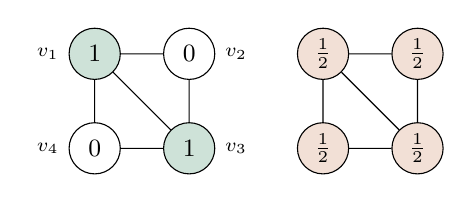
\begin{tikzpicture}[
    vtx/.style={circle, draw, minimum size=6.5mm, inner sep=0pt, font=\small}]
  \begin{scope}
    \node[vtx, fill=good!22, label={[font=\scriptsize]left:$v_1$}]  (a) at (0,1.2) {$1$};
    \node[vtx,               label={[font=\scriptsize]right:$v_2$}] (b) at (1.2,1.2) {$0$};
    \node[vtx, fill=good!22, label={[font=\scriptsize]right:$v_3$}] (c) at (1.2,0) {$1$};
    \node[vtx,               label={[font=\scriptsize]left:$v_4$}]  (d) at (0,0) {$0$};
    \draw (a) -- (b) -- (c) -- (d) -- (a) -- (c);
  \end{scope}
  \begin{scope}[xshift=2.9cm]
    \node[vtx, fill=warn!18] (a) at (0,1.2) {$\tfrac12$};
    \node[vtx, fill=warn!18] (b) at (1.2,1.2) {$\tfrac12$};
    \node[vtx, fill=warn!18] (c) at (1.2,0) {$\tfrac12$};
    \node[vtx, fill=warn!18] (d) at (0,0) {$\tfrac12$};
    \draw (a) -- (b) -- (c) -- (d) -- (a) -- (c);
  \end{scope}
\end{tikzpicture}%

    \captionof{figure}{The square with a diagonal: non-TU, yet exact. Both labellings are optimal vertices of value~2.}
    \label{fig:diag}
  \end{minipage}\hfill
  \begin{minipage}[b]{0.56\textwidth}\centering\small
    \captionof{table}{E1: exact instances out of 50 non-bipartite graphs per cell; in parentheses, those where simplex returned an integral vector.}
    \label{tab:e1}
    \begin{tabular}{@{}r*{5}{c}@{}}
      \toprule
      & \multicolumn{5}{c}{edge probability $p$} \\
      \cmidrule(l){2-6}
      $n$ & 0.05 & 0.1 & 0.2 & 0.4 & 0.7 \\
      \midrule
      10 & 32 (26) & 39 (36) & 33 (30) & 21 (12) & 0 \\
      20 & 34 (30) & 42 (41) & 11 \phantom{0}(6) & 0 & 0 \\
      40 & 46 (43) & \phantom{0}9 \phantom{0}(7) & 0 & 0 & 0 \\
      60 & 21 (11) & 0 & 0 & 0 & 0 \\
      \bottomrule
    \end{tabular}
  \end{minipage}
\end{figure}

\paragraph{Results.} The relaxation was exact on 288 of the 1,000 non-TU instances (28.8\%, Table~\ref{tab:e1}), so \textbf{TU is sufficient but not necessary} for one particular LP to be exact. Exactness was common on sparse graphs (46 of 50 at $n=40$, $p=0.05$) and disappeared on dense ones, though not monotonically: 32, 39 and 33 exact graphs for $p=0.05$, $0.1$, $0.2$ at $n=10$. On 46 exact instances simplex nevertheless returned a fractional optimal vertex, as the square with a diagonal predicts. Every fractional coordinate that simplex returned, on any instance, was exactly $\tfrac12$, as Lemma~\ref{lem:half} requires. Where the LP was not exact, the ratio $\optilp/\optlp$ mostly rose with the edge probability~$p$: the largest was $55/30 \approx 1.83$, and the mean at $n=60$, $p=0.7$ was $1.82$. Complete graphs show the extreme: on $K_n$ the all-$\tfrac12$ vector is optimal (sum the edge constraints) at $n/2$, but a cover needs $n-1$ vertices, a ratio of $2-2/n$.
\section{Recognising total unimodularity}\label{sec:recognise}

Overnight shifts show that TU must be checked, not assumed. For the VC LP the check is a bipartiteness test (Theorem~\ref{thm:bip}), $O(n+m)$ by breadth-first search; for a general matrix we compare three methods.

\subsection{Three recognition methods}\label{sec:methods}

\paragraph{Brute force.} Algorithm~\ref{alg:brute} computes the determinant of every square submatrix with exact integer arithmetic. An $m\times n$ matrix has $\sum_{k\ge1}\binom{m}{k}\binom{n}{k} = \binom{m+n}{m}-1$ square submatrices, about $4^n$ for $m=n$. A TU matrix forces the full enumeration. A non-TU matrix is rejected at the first bad submatrix, so its cost depends on where that submatrix comes in the enumeration order.

\paragraph{Ghouila-Houri.} Instead of determinants, this test asks for a signing of rows (Algorithm~\ref{alg:gh}).

\begin{theorem}[Ghouila-Houri \cite{ghouilahouri1962}]\label{thm:gh}
  A matrix $A$ is TU if and only if every subset $R$ of its rows can be split into $R^+$ and $R^-$ such that $\sum_{i\in R^+} a_i - \sum_{i\in R^-} a_i$ has every entry in $\{-1,0,1\}$, where $a_i$ is row~$i$.
\end{theorem}
\begin{proof}[Proof of ``only if'']
  This direction follows from Hoffman--Kruskal. Let $A$ be TU, $R$ a set of rows with submatrix $A_R$, and $d = \mathbf 1^\top A_R$ the vector of column sums over~$R$. The polytope $\{z\in\R^R : 0\le z\le 1,\ \lfloor d/2\rfloor \le z^\top A_R \le \lceil d/2\rceil\}$ contains $z=\tfrac12\mathbf 1$, and its constraint matrix is TU by Lemma~\ref{lem:ops}, so it has an integral vertex $z\in\{0,1\}^R$. With $R^+=\{i : z_i=1\}$, the signed sum is $2z^\top A_R - d$, which lies in $\{-1,0,1\}$ entrywise. The converse is harder, and we omit it \cite{schrijver1986}.
\end{proof}

This proves that interval matrices are TU. Order any set of rows by hour and sign them $+,-,+,\dots$ (Figure~\ref{fig:families}c): each column's $1$s among them are consecutive, so its signed sum is $0$ or $\pm1$. Checking the condition directly is still exponential: each row is omitted, positive or negative, giving $3^m$ combinations ($3^{\min(m,n)}$ after transposing if needed).

\begin{figure}[H]
  \begin{minipage}[t]{0.485\textwidth}
    \begin{algobox}{Brute-force TU test}{alg:brute}
      \Require integer matrix $A\in\Z^{m\times n}$
      \Ensure TU, or a submatrix with $|\det|>1$
      \If{some entry $a_{ij}\notin\{-1,0,1\}$}
        \State \Return not TU
      \EndIf
      \For{$k = 1,\dots,\min(m,n)$}
        \For{every $k$-set $R$ of rows}
          \For{every $k$-set $J$ of columns}
            \State $d\gets\det A_{R,J}$ \Comment{exact}
            \If{$|d|>1$}
              \State \Return not TU, with $(R,J)$
            \EndIf
          \EndFor
        \EndFor
      \EndFor
      \State \Return TU
    \end{algobox}
  \end{minipage}\hfill
  \begin{minipage}[t]{0.485\textwidth}
    \begin{algobox}{Ghouila-Houri test}{alg:gh}
      \Require $A\in\{-1,0,1\}^{m\times n}$, transposed if $m>n$
      \Ensure TU, or a row set with no valid signing
      \For{every nonempty row set $R$, by size}
        \State $\mathit{found}\gets$ false
        \For{every $\sigma\in\{\pm1\}^R$ with $\sigma_{\min R}=+1$}
          \If{$\sum_{i\in R}\sigma_i a_i\in\{-1,0,1\}^n$}
            \State $\mathit{found}\gets$ true; \textbf{break}
          \EndIf
        \EndFor
        \If{not $\mathit{found}$}
          \State \Return not TU, with $R$
        \EndIf
      \EndFor
      \State \Return TU
    \end{algobox}
  \end{minipage}
\end{figure}

\paragraph{Seymour's decomposition.} The polynomial-time route is structural. A \emph{network matrix} comes from a directed tree $T$: each arc $(u,v)$ gives a column with $\pm1$ on the tree arcs of the $u$--$v$ path in $T$, signed by direction. Network matrices are TU (interval matrices are those of a directed path). Seymour's theorem \cite{seymour1980} builds every TU matrix, up to simple operations, from network matrices, their transposes and two exceptional $5\times5$ matrices by gluing along small interfaces (1-, 2- and 3-sums), and running it in reverse gives a polynomial-time test \cite{truemper1990}. We did not implement this test: E2 runs the CMR library's implementation \cite{walter2013,cmr} and records its yes/no answer and running time, not which decomposition steps it took.

\subsection{E2: How costly is recognising TU?}\label{sec:e2}

\paragraph{Setup.}
\begin{setup}
  \item \emph{Instances:} 340 matrices with known answers: the six families of Table~\ref{tab:e2}, where the ``embedded triangle'' is a $C_3$ block in the top-left corner beside an even cycle; 12 small controls; and 40 transposed, permuted or sign-flipped copies, which must keep their parent's answer.
  \item \emph{Methods:} Algorithms~\ref{alg:brute} and~\ref{alg:gh} in Python (exact integer arithmetic); CMR~1.4 in compiled C.
  \item \emph{Measured:} answer and running time, in three runs per method and matrix with a one-second limit; for Python also \emph{algorithm time}, which excludes about 42\,ms of start-up.
\end{setup}

\paragraph{Results.} Every completed decision was correct, and every finished transformed copy kept its parent's answer. CMR decided all 340 matrices in every repetition, the largest (160 vertices, up to 3,871 rows) in about 31\,ms; most calls took 3--7\,ms, mainly start-up. The exhaustive methods hit the limit early (Table~\ref{tab:e2}; plots in Appendix~\ref{app:e2fig}). On even cycles, brute force's algorithm time grew about 21-fold per two extra rows, to $652$\,ms at order~10, where it checks 184,755 submatrices. GH grew about 9-fold per two rows, the $3^2$ factor of its row choices, and reached $153$\,ms at order~12. Where both finished, GH was faster on 151 of 160 inputs (median factor 14).

\begin{table}[H]
  \centering\small
  \caption{E2: largest size at which each method finished every input, in all three runs, within one second.}
  \label{tab:e2}
  \begin{tabular}{@{}llcrrr@{}}
    \toprule
    & & & \multicolumn{3}{c}{Largest completed size} \\
    \cmidrule(l){4-6}
    Family & TU & Sizes tested & Brute & GH & CMR \\
    \midrule
    Even cycle (order) & yes & 4--160 & 10 & 12 & all \\
    Odd cycle (order) & no & 3--159 & 9 & 11 & all \\
    Embedded triangle (order) & no & 7--131 & 35 & all & all \\
    Bipartite, $p=0.2$ and $0.6$ (vertices) & yes & 8--160 & 8 & 12 & all \\
    Interval, short and long (order) & yes & 4--32 & 10 & 10 & all \\
    Block-diagonal cycles (order) & yes & 8--96 & 8 & 12 & all \\
    \bottomrule
  \end{tabular}
\end{table}

Negative answers depend on structure. An odd cycle's only obstruction is the full matrix, so both exhaustive methods search everything first and fail at similar sizes to even cycles. The embedded triangle's obstruction is a $3\times3$ corner: GH reaches it after the one- and two-row subsets and rejected even the order-131 matrix in $290$\,ms, while brute force must first check every $2\times2$ submatrix (72.5 million at order~131) and timed out from order~67. It timed out on all three permuted copies of the order-35 matrix it had rejected, where the triangle comes later.

\section{Solving the LP: does the algorithm matter?}\label{sec:solve}

Corollary~\ref{cor:lp-exact} guarantees an integral optimal \emph{vertex}. When vertices tie, every point of the face between them is optimal, and which one a solver returns depends on the algorithm (Figure~\ref{fig:paths}).

\subsection{Where LP algorithms stop}\label{sec:algorithms}

\paragraph{The simplex method.} Simplex \cite{dantzig1951} (Algorithm~\ref{alg:simplex}) pivots between adjacent bases without worsening the objective (a \emph{degenerate} pivot changes the basis but not the vertex). With an anti-cycling rule such as Bland's \cite{bland1977} it stops at an optimal vertex, which on a TU instance is integral. Dual simplex \cite{lemke1954} keeps optimality and restores feasibility instead, also ending at a vertex. The \emph{pivot rule} chooses $j$ in line~6. Dantzig's rule, the largest $c_j-y^\top a_j$, visits all $2^n$ vertices of the Klee--Minty cube \cite{kleeminty1972}, and no rule is known to be polynomial. HiGHS \cite{huangfu2018}, which we use, defaults to weighted rules: \emph{steepest edge} \cite{forrestgoldfarb1992} in dual simplex (possibly switching to Devex) and its approximation \emph{Devex} \cite{harris1973} in primal simplex.

\paragraph{The ellipsoid method.} Khachiyan's method \cite{khachiyan1979} first put LP in P but is slow in practice, and its bound grows with the bit length $L$ (\emph{weakly} polynomial). For matrices with small integer entries, TU ones included, LP is strongly polynomial \cite{tardos1986}.

\paragraph{Interior point methods.} IPMs \cite{karmarkar1984} are polynomial ($O(n^{3.5}L)$ for Karmarkar's method) and fast in practice. A path-following IPM (Algorithm~\ref{alg:ipm}, a schematic without centrality control or a stopping test) adds a barrier $\mu\sum_i\log s_i$ on the slacks $s_i$, including those of $x\ge0$, which keeps iterates strictly inside the polyhedron, and follows the maximisers (the \emph{central path}) as $\mu\to0$. The central path ends in the relative interior of the optimal face \cite{guler1993}: at a vertex if the optimum is unique, and otherwise strictly between the extremes of every coordinate that varies over the face. A finite run stops near this point. For the VC LP on bipartite graphs, whose optimal vertices are $0/1$ covers, the IPM answer is fractional on exactly the \emph{free} vertices, those in some but not all minimum covers (Figure~\ref{fig:paths}b). Intuitively, a segment's midpoint is never an endpoint. \emph{Crossover} \cite{megiddo1991} then recovers an optimal vertex.

\begin{figure}[H]
  \begin{minipage}[t]{0.485\textwidth}
    \begin{algobox}{Simplex method}{alg:simplex}
      \Require $[A\ \ I]$, $b$, $c$; a feasible basis $B$
      \Ensure an optimal vertex, or ``unbounded''
      \Loop
        \State $x_B\gets A_B^{-1}b$,\ \ $x_j\gets 0$ for every $j\notin B$
        \State $y\gets (A_B^{-1})^{\top} c_B$ \Comment{prices}
        \If{$c_j - y^\top a_j\le 0$ for every $j\notin B$}
          \State \Return $x$ \Comment{optimal vertex}
        \EndIf
        \State pick an improving $j\notin B$ \Comment{anti-cycling rule}
        \State $d\gets A_B^{-1}a_j$ \Comment{edge direction}
        \If{$d\le 0$} \Return unbounded \EndIf
        \State $i\gets\arg\min\{x_{B_i}/d_i : d_i>0\}$ \Comment{ratio test}
        \State $B\gets B\setminus\{B_i\}\cup\{j\}$ \Comment{pivot}
      \EndLoop
    \end{algobox}
  \end{minipage}\hfill
  \begin{minipage}[t]{0.485\textwidth}
    \begin{algobox}{IPM and crossover (schematic)}{alg:ipm}
      \Require $A$, $b$, $c$; $x$ with all slacks $s(x)>0$; $\mu>0$
      \Ensure a near-optimal point; with crossover, an optimal vertex
      \While{$\mu>\varepsilon$}
        \State Newton step on $\max\ c^\top x+\mu\textstyle\sum_i\log s_i(x)$,
        \Statex \hspace{\algorithmicindent}\hspace{\algorithmicindent}shortened so that $s(x)>0$
        \State $\mu\gets\theta\mu$ \Comment{$0<\theta<1$}
      \EndWhile
      \If{crossover}
        \State find a basis near $x$ \Comment{basis recovery}
        \State $x\gets$ simplex from that basis \Comment{certify}
      \EndIf
      \State \Return $x$
    \end{algobox}
  \end{minipage}
\end{figure}

\begin{figure}[H]
  \centering
  \begin{minipage}[b]{0.38\textwidth}\centering
    % Figure~\ref{fig:paths}a: where simplex, IPM and crossover stop.
% Input by sections/05-solving-lp.tex.
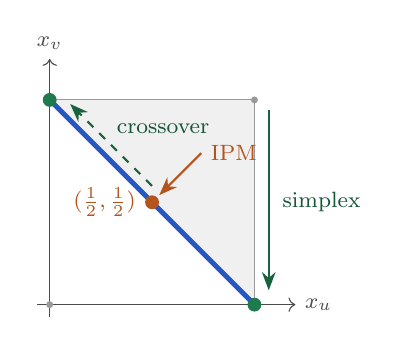
\begin{tikzpicture}[scale=2.6, font=\footnotesize,
    lat/.style={circle, fill=black!40, inner sep=0pt, minimum size=2.5pt},
    gv/.style={circle, fill=good, inner sep=0pt, minimum size=5pt},
    wv/.style={circle, fill=warn, inner sep=0pt, minimum size=5pt}]
  \fill[black!6] (1,0) -- (1,1) -- (0,1) -- cycle;
  \draw[black!40] (1,0) -- (1,1) -- (0,1);
  \draw[accent, line width=1.8pt] (1,0) -- (0,1);
  \draw[->, black!70] (-0.06,0) -- (1.2,0) node[right] {$x_u$};
  \draw[->, black!70] (0,-0.06) -- (0,1.2) node[above] {$x_v$};
  \foreach \p in {(0,0),(1,0),(0,1),(1,1)} \node[lat] at \p {};
  % simplex: from vertex (1,1) to vertex (1,0)
  \draw[good!80!black, thick, -{Stealth}] (1.07,0.95) -- (1.07,0.07);
  \node[good!70!black, anchor=west] at (1.09,0.5) {simplex};
  % IPM: central path along the diagonal to the centre of the face
  \draw[warn, thick, -{Stealth}] (0.74,0.74) -- (0.535,0.535);
  \node[warn, anchor=west] at (0.74,0.74) {IPM};
  \node[wv] at (0.5,0.5) {};
  \node[warn, anchor=east, inner sep=2pt] at (0.45,0.5) {$(\tfrac12,\tfrac12)$};
  % crossover: along the face to a vertex
  \draw[good!80!black, thick, dashed, -{Stealth}] (0.5,0.58) -- (0.1,0.98);
  \node[good!70!black, anchor=west] at (0.28,0.86) {crossover};
  \node[gv] at (1,0) {};
  \node[gv] at (0,1) {};
\end{tikzpicture}%
\\[2pt]
    (a) VC LP of one edge $\{u,v\}$
  \end{minipage}\hfill
  \begin{minipage}[b]{0.58\textwidth}\centering
    % Figure~\ref{fig:paths}b: tree with free vertices.
% Input by sections/05-solving-lp.tex.
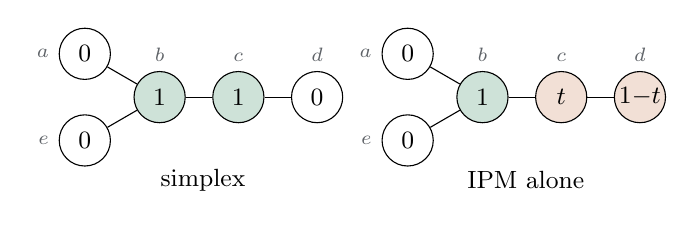
\begin{tikzpicture}[
    vtx/.style={circle, draw, minimum size=6.5mm, inner sep=0pt, font=\small},
    nm/.style={font=\scriptsize, text=muted}]
  \foreach \xs/\title/\cv/\dv/\cf/\df in {
      0/{simplex}/{$1$}/{$0$}/{good!22}/{white},
      4.1/{IPM alone}/{$t$}/{$1{-}t$}/{warn!18}/{warn!18}} {
    \begin{scope}[xshift=\xs cm]
      \node[vtx, label={[nm]left:$a$}]  (a) at (0, 0.55) {$0$};
      \node[vtx, label={[nm]left:$e$}]  (e) at (0,-0.55) {$0$};
      \node[vtx, fill=good!22, label={[nm]above:$b$}] (b) at (0.95,0) {$1$};
      \node[vtx, fill=\cf, label={[nm]above:$c$}] (c) at (1.95,0) {\cv};
      \node[vtx, fill=\df, label={[nm]above:$d$}] (d) at (2.95,0) {\dv};
      \draw (a) -- (b) -- (e); \draw (b) -- (c) -- (d);
      \node[font=\small] at (1.5,-1.05) {\title};
    \end{scope}
  }
\end{tikzpicture}%
\\[2pt]
    (b) a tree with free vertices $c$ and $d$; $0<t<1$
  \end{minipage}
  \caption{Which optimal point each algorithm returns. (a)~The optimal face (thick) joins the covers $(1,0)$ and $(0,1)$. Simplex walks along edges to a vertex; the IPM follows the central path to the face's centre $(\tfrac12,\tfrac12)$; crossover moves on to a vertex. (b)~$b$ is in every minimum cover, $a$ and $e$ in none, $c$ and $d$ in some (free). Simplex returns $\{b,c\}$ or $\{b,d\}$; IPM alone is fractional on exactly $c$ and~$d$.}
  \label{fig:paths}
\end{figure}

\subsection{E3: Does the LP algorithm matter?}\label{sec:e3}

\paragraph{Setup.}
\begin{setup}
  \item \emph{Instances:} the 18 bipartite (so TU), unit-cost graphs of Table~\ref{tab:e3}: symmetric families (every vertex free), three controls with one minimum cover and three KONECT networks \cite{kunegis2013}.
  \item \emph{Methods:} dual simplex, IPM with crossover, and IPM alone (HiGHS~1.15.1), all with presolve off, so that HiGHS's clean-up pass cannot settle ties before the algorithm runs.
  \item \emph{Measured:} which coordinates are fractional, meaning more than $10^{-6}$ from an integer, compared with the free vertices found by König's construction (Algorithm~\ref{alg:free}).
  \item \emph{Checks:} free set confirmed by a second method on the 16 graphs with $n\le 2{,}000$ (Table~\ref{tab:instances}).
\end{setup}

\paragraph{Results.} The prediction held on all 18 instances (Table~\ref{tab:e3}). Simplex and IPM with crossover always returned integral vertices. IPM alone was fractional on exactly the free vertices: the same set, not just the same number, up to the 7,934 free vertices of the arXiv graph. The tolerance does not matter: every free coordinate was at least $0.018$ from an integer, and every other one within $3.4\times10^{-8}$. On the symmetric families IPM returned exactly $\tfrac12$ everywhere: every edge lies in a perfect matching, so every edge is tight on the whole optimal face, the segment between the two sides, whose centre is all-$\tfrac12$. On the real graphs free values ranged from $0.019$ to $0.981$, and only 5--11\% were within $10^{-4}$ of $\tfrac12$ (Lemma~\ref{lem:half} is about vertices, and the IPM point is not one). Ties are common in real data: 10\%, 25\% and 20\% of vertices were free.

\begin{figure}[H]
  \begin{minipage}[c]{0.475\textwidth}
    \begin{algobox}{Free vertices via König}{alg:free}
      \Require bipartite graph $G$
      \State $M\gets$ maximum matching \cite{hopcroft1973}
      \State $O\gets$ vertices unmatched by $M$
      \While{a neighbour $w$ of $O$ has $M(w)\notin O$}
        \State $O\gets O\cup\{M(w)\}$
      \EndWhile
      \State \Return $\{v \text{ matched}: v\notin O,\ M(v)\notin O\}$
    \end{algobox}
  \end{minipage}\hfill
  \begin{minipage}[c]{0.495\textwidth}\small\raggedright
    $O$ is the set of vertices in \emph{no} minimum cover. A minimum cover takes one endpoint of each matching edge (König), so:
    \begin{itemize}[leftmargin=1.2em, itemsep=0pt, parsep=0pt, topsep=1pt]
      \item unmatched vertices are in $O$;
      \item neighbours $w$ of $O$ are in every cover, so $M(w)\in O$;
      \item the rest are free: no edge joins them to $O$, or $O$ to $O$ ($M$ is maximum), so the neighbours of $O$ plus the left (or right) ends of the other matching edges are two covers of size $|M|$.
    \end{itemize}
    Figure~\ref{fig:paths}b: $O=\{e,a\}$, free $=\{c,d\}$.
  \end{minipage}
\end{figure}

\begin{table}[H]
  \centering\small
  \caption{E3: predicted free vertices and the number of fractional coordinates returned by each configuration. In every row, the fractional coordinates of IPM alone are exactly the free vertices.}
  \label{tab:e3}
  \begin{tabular}{@{}lrrrrr@{}}
    \toprule
    & & & \multicolumn{3}{c}{Fractional coordinates} \\
    \cmidrule(l){4-6}
    Instances & Vertices $n$ & Free & Simplex & IPM + crossover & IPM alone \\
    \midrule
    $C_4,\ C_{20},\ C_{100},\ C_{1000}$ & 4--1,000 & $n$ & 0 & 0 & $n$ \\
    $K_{3,3}$ to $K_{100,100}$ & 6--200 & $n$ & 0 & 0 & $n$ \\
    grids $4\times4$ to $100\times100$ & 16--10,000 & $n$ & 0 & 0 & $n$ \\
    controls ($K_{3,4}$, $K_{30,31}$, Davis \cite{davis1941}) & 7--61 & 0 & 0 & 0 & 0 \\
    Unicode languages & 868 & 90 & 0 & 0 & 90 \\
    Crime & 1,380 & 348 & 0 & 0 & 348 \\
    arXiv cond-mat \cite{newman2001} & 38,741 & 7,934 & 0 & 0 & 7,934 \\
    \bottomrule
  \end{tabular}
\end{table}

So the algorithm matters for the \emph{answer} even when the LP is exact. Rounding the IPM point at $\tfrac12$ always gave a valid cover, but of size exactly $2\optilp$ on every symmetric instance and $1.6$--$3.3\%$ above the optimum on the real graphs. Crossover turns ``the LP is exact'' into ``the solver's answer is exact'', at a cost: IPM needed 5--17 iterations on every instance, while crossover added up to 6,896 (on the $100\times100$ grid).

\subsection{E4: Should we just solve the LP?}\label{sec:e4}

\paragraph{Setup.}
\begin{setup}
  \item \emph{Instances:} max-flow on random networks and grids; bipartite matching on random graphs and E3's real graphs; shift scheduling. Up to 10,000 nodes or vertices per side (Table~\ref{tab:instances}).
  \item \emph{Methods:} HiGHS dual and primal simplex against Edmonds--Karp \cite{edmondskarp1972} and Dinic \cite{dinitz1970} (flow) and Hopcroft--Karp \cite{hopcroft1973} (matching), each in compiled (SciPy) and pure-Python (networkx) code to separate algorithm from language; for scheduling, the LP against HiGHS B\&B.
  \item \emph{Measured:} for flow and matching, solve time without model building (under 5\,ms); for scheduling, time including it. Median of up to three runs on one laptop; runs over 2\,s not repeated.
\end{setup}

\paragraph{Results.} Every method agreed on all 13 flow and matching instances, and both simplex variants returned integral optima. The specialised algorithms were far faster (Figure~\ref{fig:e4}). On the 10,000-node network the LP took 10.1\,s (dual) or 4.7\,s (primal) against 15.5\,ms for compiled Dinic, a factor of 300--650; on the arXiv matching instance it took 0.31\,s against 2.4\,ms for Hopcroft--Karp. From 1,000 to 10,000 nodes, dual simplex time grew 120-fold and Dinic's 13-fold, and the pivot count 15-fold. One possible reason, which we did not measure, is degeneracy: flow LPs have many bases per vertex, so many pivots may not move the vertex, while the specialised algorithms run a few graph searches per round. Implementation matters as much as the algorithm: pure-Python Dinic took 19.4\,s on the largest network, longer than the LP. Ratios vary by instance, simplex variant and run (Appendix~\ref{app:e4}): compiled specialised code always won, by 2--3 orders of magnitude on the largest random instances but 13--31 times on grids.

For day-shift scheduling the LP was integral and equal to the ILP optimum on all 15 instances, and 3--16 times faster than the ILP solver. (Interval matrices also reduce to min-cost flow \cite{veinott1962a,veinott1962b}, which we did not try.) With overnight shifts, the LP was fractional and strictly below the integer optimum on 24 of 200 instances (12\%), by 0.33 to 0.75 staff, and the integer optimum was always the LP value rounded up: losing TU allows $\optlp<\optilp$ but does not force it, as in E1.

\begin{figure}[H]
  \centering
  % Figure~\ref{fig:e4}: E4 solve times.
% Data copied from experiments/E4/results/flow.csv and matching.csv (median times).
% Input by sections/05-solving-lp.tex.
\pgfplotsset{timeplot/.style={
    width=0.5\textwidth, height=4.3cm,
    ymin=1e-5, ymax=60, xmin=70, xmax=14000,
    grid=major, grid style={black!10},
    axis line style={black!45}, tick style={black!45},
    tick label style={font=\scriptsize}, label style={font=\small},
    title style={font=\small, yshift=-4pt},
    ylabel={solve time (s)}, ylabel style={yshift=-2pt},
    every axis plot/.append style={line width=1pt, mark size=2pt}}}
\tikzset{dl/.style={font=\scriptsize, text=black, inner sep=1.5pt}}
\begin{tikzpicture}
  \begin{axis}[xmode=log, ymode=log, timeplot, title={(a) Max-flow, random networks}, xlabel={nodes}]
    \addplot[series1, mark=*] coordinates {(100,0.002710) (1000,0.083347) (3000,0.498343) (10000,10.126597)};
    \addplot[series2, mark=square*] coordinates {(100,0.0001367) (1000,0.001174) (3000,0.003746) (10000,0.015489)};
    \addplot[series3, mark=triangle*, mark size=2.6pt] coordinates {(100,0.001876) (1000,0.124375) (3000,2.781808) (10000,19.408298)};
    \node[dl, anchor=north west] at (axis cs:3000,0.40) {LP};
    \node[dl, anchor=south east] at (axis cs:2600,2.9) {Dinic, Python};
    \node[dl, anchor=north] at (axis cs:3000,0.0026) {Dinic, compiled};
  \end{axis}
\end{tikzpicture}\hfill
\begin{tikzpicture}
  \begin{axis}[xmode=log, ymode=log, timeplot, title={(b) Matching, random bipartite graphs}, xlabel={vertices per side}]
    \addplot[series1, mark=*] coordinates {(100,0.0011298) (1000,0.0340516) (10000,1.1374447)};
    \addplot[series2, mark=square*] coordinates {(100,0.0000245) (1000,0.000382) (10000,0.0079618)};
    \addplot[series3, mark=triangle*, mark size=2.6pt] coordinates {(100,0.000504) (1000,0.011560) (10000,0.228602)};
    \node[dl, anchor=south east] at (axis cs:1000,0.040) {LP};
    \node[dl, anchor=north west] at (axis cs:1100,0.0095) {HK, Python};
    \node[dl, anchor=north] at (axis cs:1000,0.00028) {HK, compiled};
  \end{axis}
\end{tikzpicture}\\[2pt]
{\small
 \legline{series1}{*}~LP, HiGHS dual simplex\qquad
 \legline{series2}{square*}~compiled (SciPy)\qquad
 \legline{series3}{triangle*}~pure Python (networkx)}%

  \caption{E4: solve times (log--log) of the LP against Dinic (max-flow) and Hopcroft--Karp (HK, matching). Primal simplex, Edmonds--Karp, grids and real graphs are in Appendix~\ref{app:e4}.}
  \label{fig:e4}
\end{figure}

\section{Conclusion}\label{sec:conclusion}

\begin{itemize}[topsep=0pt]
  \item \textbf{When.} If $A$ is TU and $b$ integral, every vertex is integral (Hoffman--Kruskal): hence integral flows, König's theorem and shift scheduling. TU is sufficient but not necessary: the VC LP was exact on 28.8\% of our non-TU graphs (E1), with half-integral vertices.
  \item \textbf{How to recognise.} A known structure can make the test trivial (bipartiteness). On cycles and several TU families exhaustive recognition became impractical around order 10--12, although small, early obstructions let it reject much larger matrices; CMR's implementation of Seymour's test decided all 340 inputs (E2).
  \item \textbf{Does the algorithm matter.} Yes. TU guarantees integral vertices, not integral optimal points: simplex and IPM with crossover returned integral answers, while IPM alone was fractional on exactly the free vertices (E3). An exact LP is not always the best tool: compiled flow and matching code was always faster, by 2--3 orders of magnitude on the largest random instances, while for shift scheduling the LP was the practical route (E4).
\end{itemize}

\paragraph{Limitations.} All LPs were solved with HiGHS, most instances were synthetic and unit-cost, our timings partly compare implementations (Python against C), and CMR's times were too close to its start-up cost to show scaling. We proved one direction of Hoffman--Kruskal and Ghouila-Houri, and saw only CMR's answers to Seymour's test, not its decomposition steps.

\paragraph{Beyond our scope.} A system $Ax\le b$ is \emph{totally dual integral} if the dual LP has an integral optimum for every integral objective with a finite optimum; with $b$ integral, it defines an integral polyhedron even when $A$ is not TU \cite{edmonds1977}. In the same spirit, Edmonds's matching polytope \cite{edmonds1965} describes matchings in non-bipartite graphs, where the incidence matrix is not TU. Current research bounds subdeterminants by a constant $\Delta$ instead of~$1$: integer programs with $\Delta=2$ (bimodular) are solvable in strongly polynomial time \cite{artmann2017}, as are $\Delta$-modular programs with at most two nonzeros per row, for fixed $\Delta$ \cite{fiorini2021}. Progress on strictly $\Delta$-modular programs continues \cite{nagele2024}, but to our knowledge it is open whether every fixed $\Delta$ admits a polynomial-time algorithm.

\label{end-of-main-body}

% References start on a new page so that the main body is exactly pages 1-10.
\clearpage
\bibliographystyle{plainnat}
\bibliography{references}

\clearpage
\appendix
\section{Reproducing the experiments}\label{app:repro}

Each experiment lives in its own folder \texttt{experiments/E1}--\texttt{E4} of the repository, with one script, a README that documents the method in full, the input data and the saved results. The pinned versions highspy~1.15.1, networkx~3.6.1, NumPy~2.5.4 and SciPy~1.18.1 (\texttt{pip install -r requirements.txt}) are the recommended environment for reproducing all four. The saved results record their own environments: E1 ran with Python~3.12.14, NumPy~2.3.5 and SciPy~1.17.0 (whose bundled HiGHS is 1.8.0), E3 and E4 with highspy~1.15.1 and NumPy~2.4.1. A rerun of E1 with the pinned versions (SciPy's bundled HiGHS~1.12.0) on 12~November~2026 gave identical LP and ILP values, exactness, integrality, half-integral counts and LP iteration counts on all 1,012 instances; only B\&B node counts, which the report does not use, differed (on 114), apart from rounding-level differences in the B\&B dual bound. The rerun and a row-by-row comparison are saved in \texttt{experiments/E1/results/rerun-pinned-2026-11-12}. E4's README records the same agreement for its rerun. Timings differ between machines and runs. E2 additionally needs the CMR library~1.4.0, built from source (commit \texttt{0c42a44}; build steps in the E2 README), and its figures need Matplotlib (\texttt{requirements-analysis.txt}).

\begin{table}[H]
  \centering\footnotesize
  \caption{One command per experiment. Run times are from Apple~M-series laptops.}
  \label{tab:commands}
  \begin{tabular}{@{}lll@{}}
    \toprule
    & Command (run inside the experiment's folder) & Approximate run time \\
    \midrule
    E1 & \texttt{python3 e1.py} \quad (exhaustive self-test: \texttt{python3 e1.py -{}-check}) & 45\,s \\
    E2 & \texttt{python3 e2.py check -{}-with-cmr -{}-cmr PATH} & seconds \\
       & \texttt{python3 e2.py run -{}-cmr PATH -{}-time-limit 1 -{}-output results/NEW} & 20\,min \\
       & \texttt{python3 analyse.py results/main\_run -{}-plots} \quad (no recognition rerun) & seconds \\
    E3 & \texttt{python3 e3.py} & 1\,min \\
    E4 & \texttt{python3 e4.py} \quad (B\&B node check: \texttt{python3 e4.py -{}-node-check}) & 75\,s \\
    \bottomrule
  \end{tabular}
\end{table}

\paragraph{Solver settings.} Table~\ref{tab:settings} lists the settings that affect results. In E3, \emph{presolve} (a clean-up pass HiGHS runs before the main algorithm) is switched off. On graphs with a leaf $u$ attached to $v$, presolve fixes $x_u=0$ and $x_v=1$ by itself, which settles exactly the ties that E3 studies before simplex or IPM sees them. With presolve on, the experiment would partly measure presolve rather than the algorithms. E1 switches LP presolve off for the same reason, so that the reported vertex is the one simplex chose. No experiment sets a pivot rule, so HiGHS uses its defaults (\texttt{simplex\_dual\_edge\_weight\_strategy} and \texttt{simplex\_primal\_edge\_weight\_strategy} are both $-1$, ``choose''): steepest edge in dual simplex, with a possible switch to Devex, and Devex in primal simplex, as set in \texttt{HEkkDual.cpp} and \texttt{HEkkPrimal.cpp} of HiGHS~1.15.1. SciPy's default in E1 passes the same choice to HiGHS.

\begin{table}[H]
  \centering\small
  \caption{Solver settings for each experiment.}
  \label{tab:settings}
  \begin{tabular}{@{}lp{0.80\textwidth}@{}}
    \toprule
    E1 & LP: SciPy \texttt{linprog(method="highs-ds")} (dual simplex), presolve off, primal and dual feasibility tolerance $10^{-8}$. ILP: SciPy \texttt{milp} (HiGHS B\&B), presolve on, relative gap $0$, 30\,s limit (never reached). Graph seed 20261102. \\
    E2 & Brute force and GH in a fresh Python process per call; CMR as \texttt{cmr-tu - -{}-algo decomposition -{}-stats -{}-time-limit 1}. One-second wall-clock limit, three repetitions, method order shuffled per input (seed 20261108). \\
    E3 & HiGHS~1.15.1 via \texttt{highspy}: \texttt{simplex\_strategy=1} (dual simplex); \texttt{solver="ipm"} with \texttt{run\_crossover} on or off. Presolve off in all three. Fractional means more than $10^{-6}$ from an integer; times are medians of three solves. \\
    E4 & Dual (\texttt{simplex\_strategy=1}) and primal (\texttt{simplex\_strategy=4}) simplex with default presolve; ILPs with HiGHS defaults; node check with presolve off and \texttt{mip\_heuristic\_effort=0}. Seed 4234. Medians of up to three runs (a run over 2\,s is not repeated). \\
    \bottomrule
  \end{tabular}
\end{table}

\paragraph{Instances and checks.} Table~\ref{tab:instances} gives the instance details and correctness checks that the main text only summarises.

\begin{table}[H]
  \centering\small
  \caption{Instances and correctness checks for each experiment.}
  \label{tab:instances}
  \begin{tabular}{@{}lp{0.80\textwidth}@{}}
    \toprule
    E1 & LP optima are certified by exact rational primal--dual pairs and non-TU claims by an odd cycle (determinant~2), and ILP optima are proven by HiGHS with zero gap and checked by enumeration for $n\le 12$. Twelve controls with known optima (including $C_3$, $C_4$, the square with a diagonal and $K_8$) all passed. \\
    E2 & Each call ran in a fresh process (3,060 calls). Algorithm~\ref{alg:brute} computes determinants by Bareiss elimination on exact integers. CMR is timed end to end only, so it has no algorithm time. \\
    E3 & Symmetric families: even cycles, complete bipartite graphs $K_{k,k}$ and square grids of even side. Controls: $K_{3,4}$, $K_{30,31}$ and the 32-vertex Davis Southern Women graph \cite{davis1941}. Real networks from KONECT \cite{kunegis2013}: countries--languages (Unicode, 868 vertices), people--crimes (Crime, 1,380) and authors--papers (arXiv condensed matter \cite{newman2001}, 38,741). For graphs with at most 2,000 vertices the free set was also computed by minimising and maximising each $x_v$ over the optimal face; the two methods always agreed. Rounding the IPM point selects coordinates of at least $\tfrac12-10^{-6}$. \\
    E4 & Max-flow: random networks with 100 to 10,000 nodes (about five arcs per node, with a super-source and super-sink each joined to 5\% of the nodes) and grids from $10\times10$ to $70\times70$, with integer capacities 1--100. Matching: random bipartite graphs with 100 to 10,000 vertices per side (three edges per vertex) and E3's three real graphs. Shift scheduling: day shifts of 4, 6 or 8 hours over horizons of 24 to 672 hours, with demand 1--20 staff per hour (15 instances), and 200 random 24-hour instances whose shifts may wrap past midnight. \\
    \bottomrule
  \end{tabular}
\end{table}

\section{Full E4 timings}\label{app:e4}

Tables~\ref{tab:e4flow}--\ref{tab:e4sched} give the committed E4 run (MacBook Air, Apple arm64, Python~3.13). For flow and matching, LP times are solve times; building the LP model in Python took under 5\,ms on every instance. Scheduling times (Table~\ref{tab:e4sched}) include building the model, for both the LP and the ILP. SciPy is compiled code; networkx is pure Python. All methods returned the same optimal value on every instance, both LP solutions were integral, and each König cover had the size of the matching. Ratios between methods varied between runs (compiled Edmonds--Karp against Dinic: 37-fold in this run, 16-fold in a rerun), so exact ratios are indicative only. In this run, compiled specialised code was faster than the LP on every instance: by 2--3 orders of magnitude on the largest random instances, but only 13--31 times on grids (dual simplex against Dinic). B\&B node counts did not separate day shifts from overnight shifts: HiGHS solved every scheduling instance at the root node, even with presolve and primal heuristics switched off.

\begin{table}[H]
  \centering\small
  \caption{E4: max-flow, LP against compiled code. EK = Edmonds--Karp.}
  \label{tab:e4flow}
  \begin{tabular}{@{}lrrrrrr@{}}
    \toprule
    Instance & Arcs & Max flow & LP dual & LP primal & SciPy EK & SciPy Dinic \\
    \midrule
    random $n=100$ & 510 & 145 & 2.7\,ms & 1.6\,ms & 0.1\,ms & 0.1\,ms \\
    random $n=1{,}000$ & 5,100 & 2,283 & 83\,ms & 51\,ms & 2.8\,ms & 1.2\,ms \\
    random $n=3{,}000$ & 15,300 & 7,045 & 498\,ms & 497\,ms & 57\,ms & 3.7\,ms \\
    random $n=10{,}000$ & 51,000 & 24,757 & 10.13\,s & 4.70\,s & 576\,ms & 15.5\,ms \\
    grid $10\times10$ & 380 & 211 & 1.6\,ms & 1.7\,ms & 0.1\,ms & 0.1\,ms \\
    grid $30\times30$ & 3,540 & 916 & 29\,ms & 21\,ms & 2.5\,ms & 1.3\,ms \\
    grid $70\times70$ & 19,460 & 2,232 & 599\,ms & 524\,ms & 78\,ms & 19\,ms \\
    \bottomrule
  \end{tabular}
\end{table}

\begin{table}[H]
  \centering\small
  \caption{E4: max-flow, pure-Python (networkx) implementations, same instances as Table~\ref{tab:e4flow}.}
  \label{tab:e4flownx}
  \begin{tabular}{@{}lrrr@{}}
    \toprule
    Instance & LP dual & nx EK & nx Dinic \\
    \midrule
    random $n=100$ & 2.7\,ms & 1.1\,ms & 1.9\,ms \\
    random $n=1{,}000$ & 83\,ms & 31\,ms & 124\,ms \\
    random $n=3{,}000$ & 498\,ms & 320\,ms & 2.78\,s \\
    random $n=10{,}000$ & 10.13\,s & 2.46\,s & 19.41\,s \\
    grid $10\times10$ & 1.6\,ms & 4.7\,ms & 6.2\,ms \\
    grid $30\times30$ & 29\,ms & 252\,ms & 199\,ms \\
    grid $70\times70$ & 599\,ms & 5.73\,s & 3.99\,s \\
    \bottomrule
  \end{tabular}
\end{table}

\begin{table}[H]
  \centering\small
  \caption{E4: bipartite matching. HK = Hopcroft--Karp. The matching size equals the size of the König cover and the VC LP optimum.}
  \label{tab:e4match}
  \begin{tabular}{@{}lrrrrrr@{}}
    \toprule
    Instance & Edges & Matching & LP dual & LP primal & SciPy HK & nx HK \\
    \midrule
    random, 100 per side    & 300    & 91     & 1.1\,ms & 1.2\,ms & $<0.1$\,ms & 0.5\,ms \\
    random, 1,000 per side  & 3,000  & 923    & 34\,ms  & 36\,ms  & 0.4\,ms    & 12\,ms \\
    random, 10,000 per side & 30,000 & 9,274  & 1.14\,s & 1.13\,s & 8.0\,ms    & 229\,ms \\
    Unicode languages       & 1,255  & 188    & 2.3\,ms & 2.3\,ms & $<0.1$\,ms & 0.7\,ms \\
    Crime                   & 1,476  & 451    & 3.7\,ms & 3.6\,ms & 0.1\,ms    & 2.8\,ms \\
    arXiv cond-mat          & 58,595 & 12,652 & 307\,ms & 308\,ms & 2.4\,ms    & 87\,ms \\
    \bottomrule
  \end{tabular}
\end{table}

\begin{table}[H]
  \centering\small
  \caption{E4: day-shift scheduling (median over five demand profiles; times include building the model). Every ILP finished at the root node.}
  \label{tab:e4sched}
  \begin{tabular}{@{}rrrrr@{}}
    \toprule
    Horizon & Shifts & LP = ILP, LP integral & LP time & ILP time \\
    \midrule
    24\,h  & 57    & 5 of 5 & 0.2\,ms & 3.2\,ms \\
    168\,h & 489   & 5 of 5 & 1.0\,ms & 4.6\,ms \\
    672\,h & 2,001 & 5 of 5 & 4.3\,ms & 14.3\,ms \\
    \bottomrule
  \end{tabular}
\end{table}

\begin{landscape}
\section{E2 scaling plots}\label{app:e2fig}

Figure~\ref{fig:e2} shows how the three recognisers scale on the cycle families and the embedded triangle, the inputs summarised in Table~\ref{tab:e2}.

\begin{figure}[H]
  \centering
  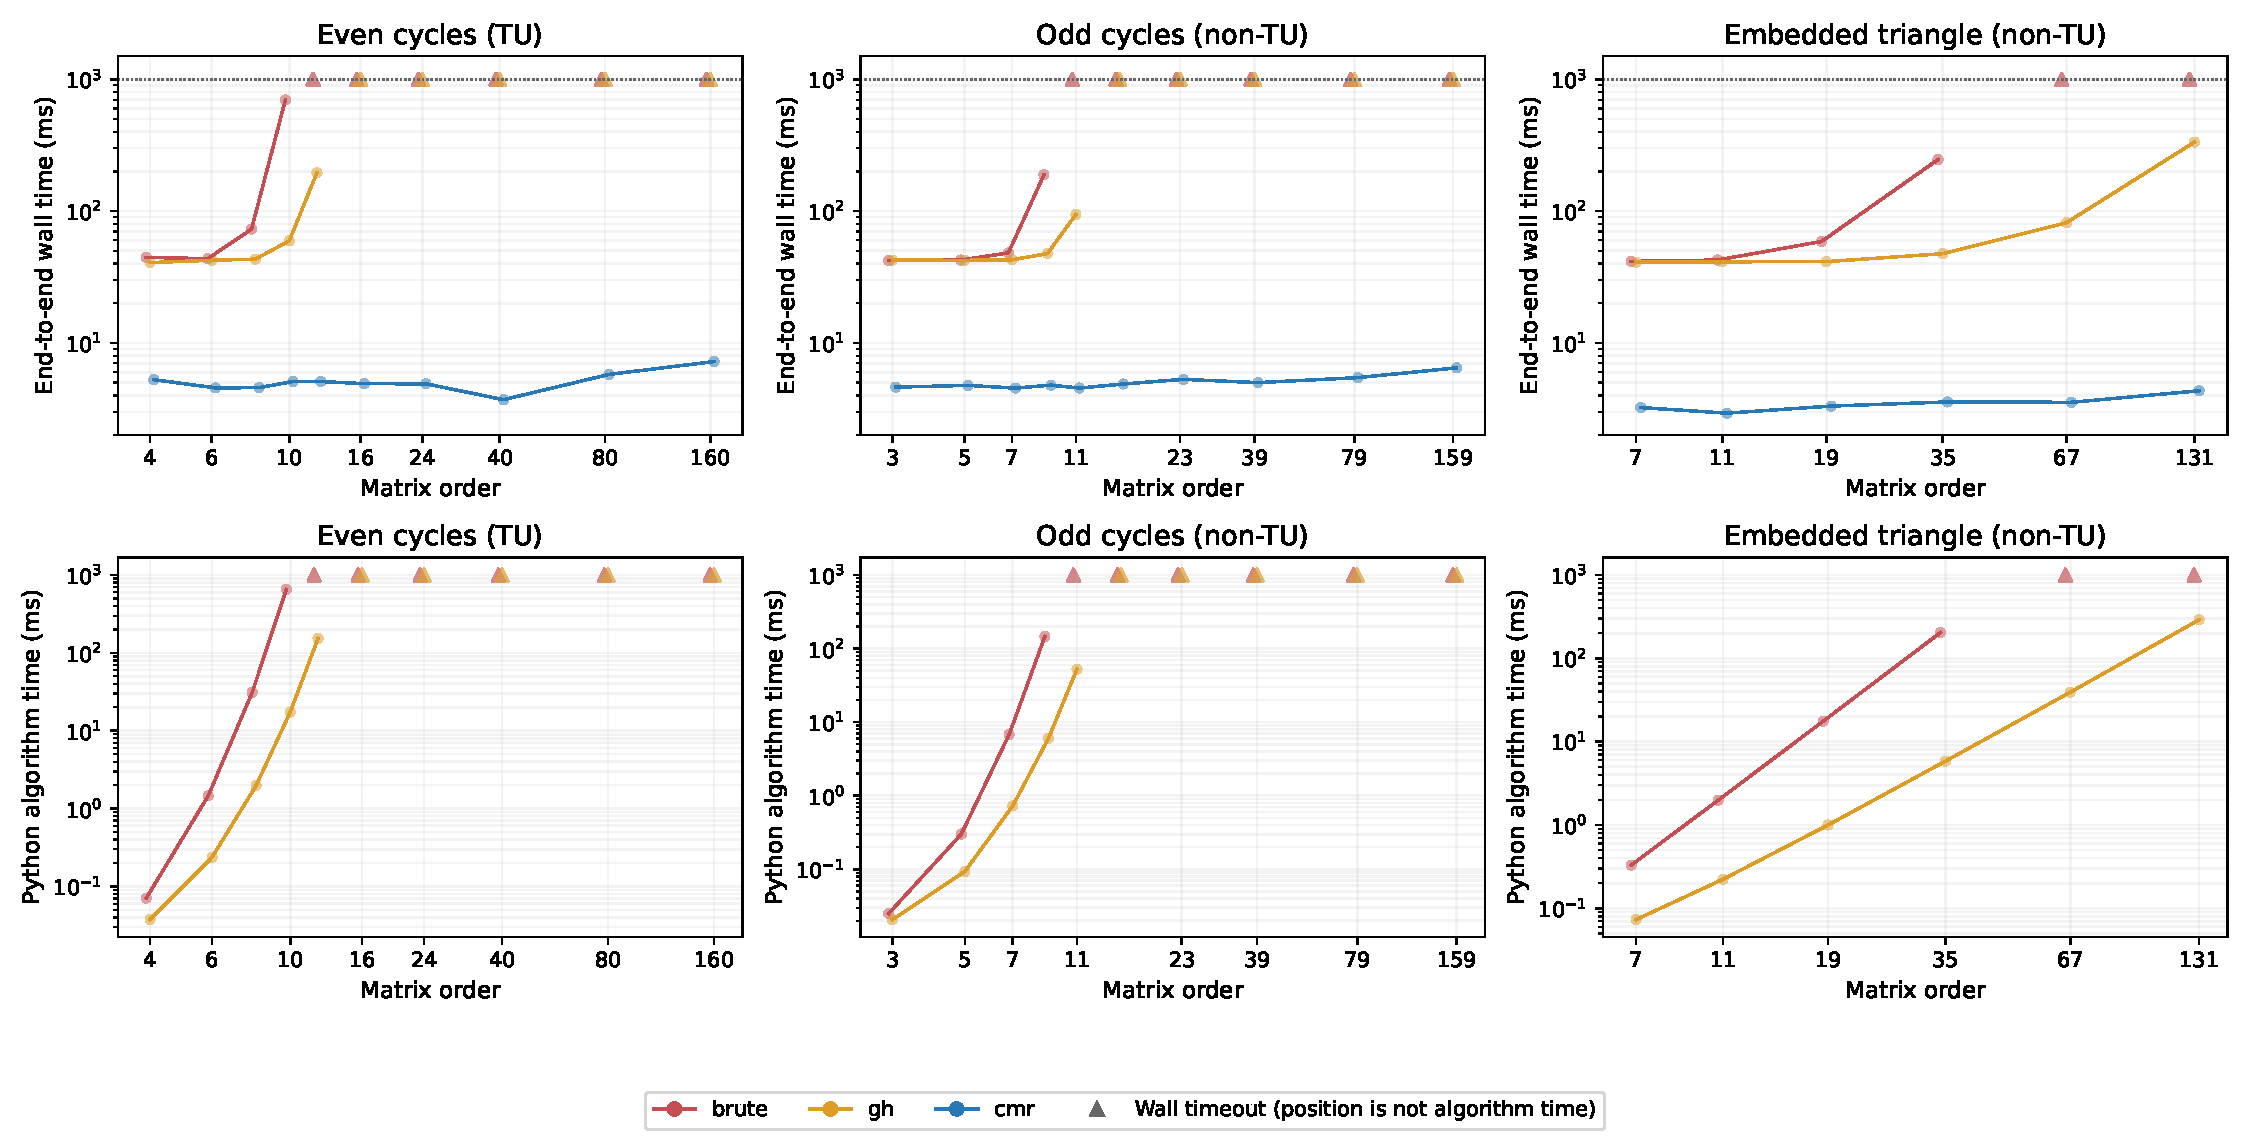
\includegraphics[width=\linewidth,height=0.78\textheight,keepaspectratio]{figures/e2-scaling.pdf}
  \caption{E2 scaling on cycles and the embedded triangle (from \texttt{experiments/E2/analysis}). Top row: end-to-end wall time for all three methods. Bottom row: algorithm time for brute force and GH, without Python start-up; CMR has no comparable internal time. Triangles mark one-second timeouts; their height is not a measured time. Figures for the other families are in the repository.}
  \label{fig:e2}
\end{figure}
\end{landscape}


% Flush all floats so that the AI Disclosure comes last.
\clearpage
\section*{AI Disclosure}
\addcontentsline{toc}{section}{AI Disclosure}

We used AI tools throughout this project under the group's direction. OpenAI Codex assisted with E1 and E2, including code, synthetic input generation, building CMR, benchmark execution, analysis, figures and documentation. Claude (Anthropic), mostly through Claude Code, assisted with E3 and E4 code and documentation, reviewed all four experiments, checked reference details against Crossref and publisher records, and drafted this report, including pseudocode and figures, from our notes and saved results. AI tools also helped draft parts of the trailer slides, scripts and notes. Reported experimental numbers come from code and saved outputs in our repository. The group has reviewed the AI-assisted material and takes responsibility for every definition, claim, proof and line of code.


\end{document}
